\section{Results}
\label{prism:sec:results}
Our algorithm is implemented in C++ and uses Eigen \cite{eigenweb} for the linear algebra routines, CGAL \revision{\cite{cgal2008computational}} and Geogram \cite{levy2015geogram} for predicates and spatial searching, and libigl \cite{jacobson2016libigl} for basic geometry processing routines.
We run our experiments on cluster nodes with a Xeon E5-2690 v2 @ 3.00GHz.
The reference implementation used to generate the results is attached to the submission and will be released as an open-source project.

\paragraph{Robustness}

\begin{figure}
    \centering
    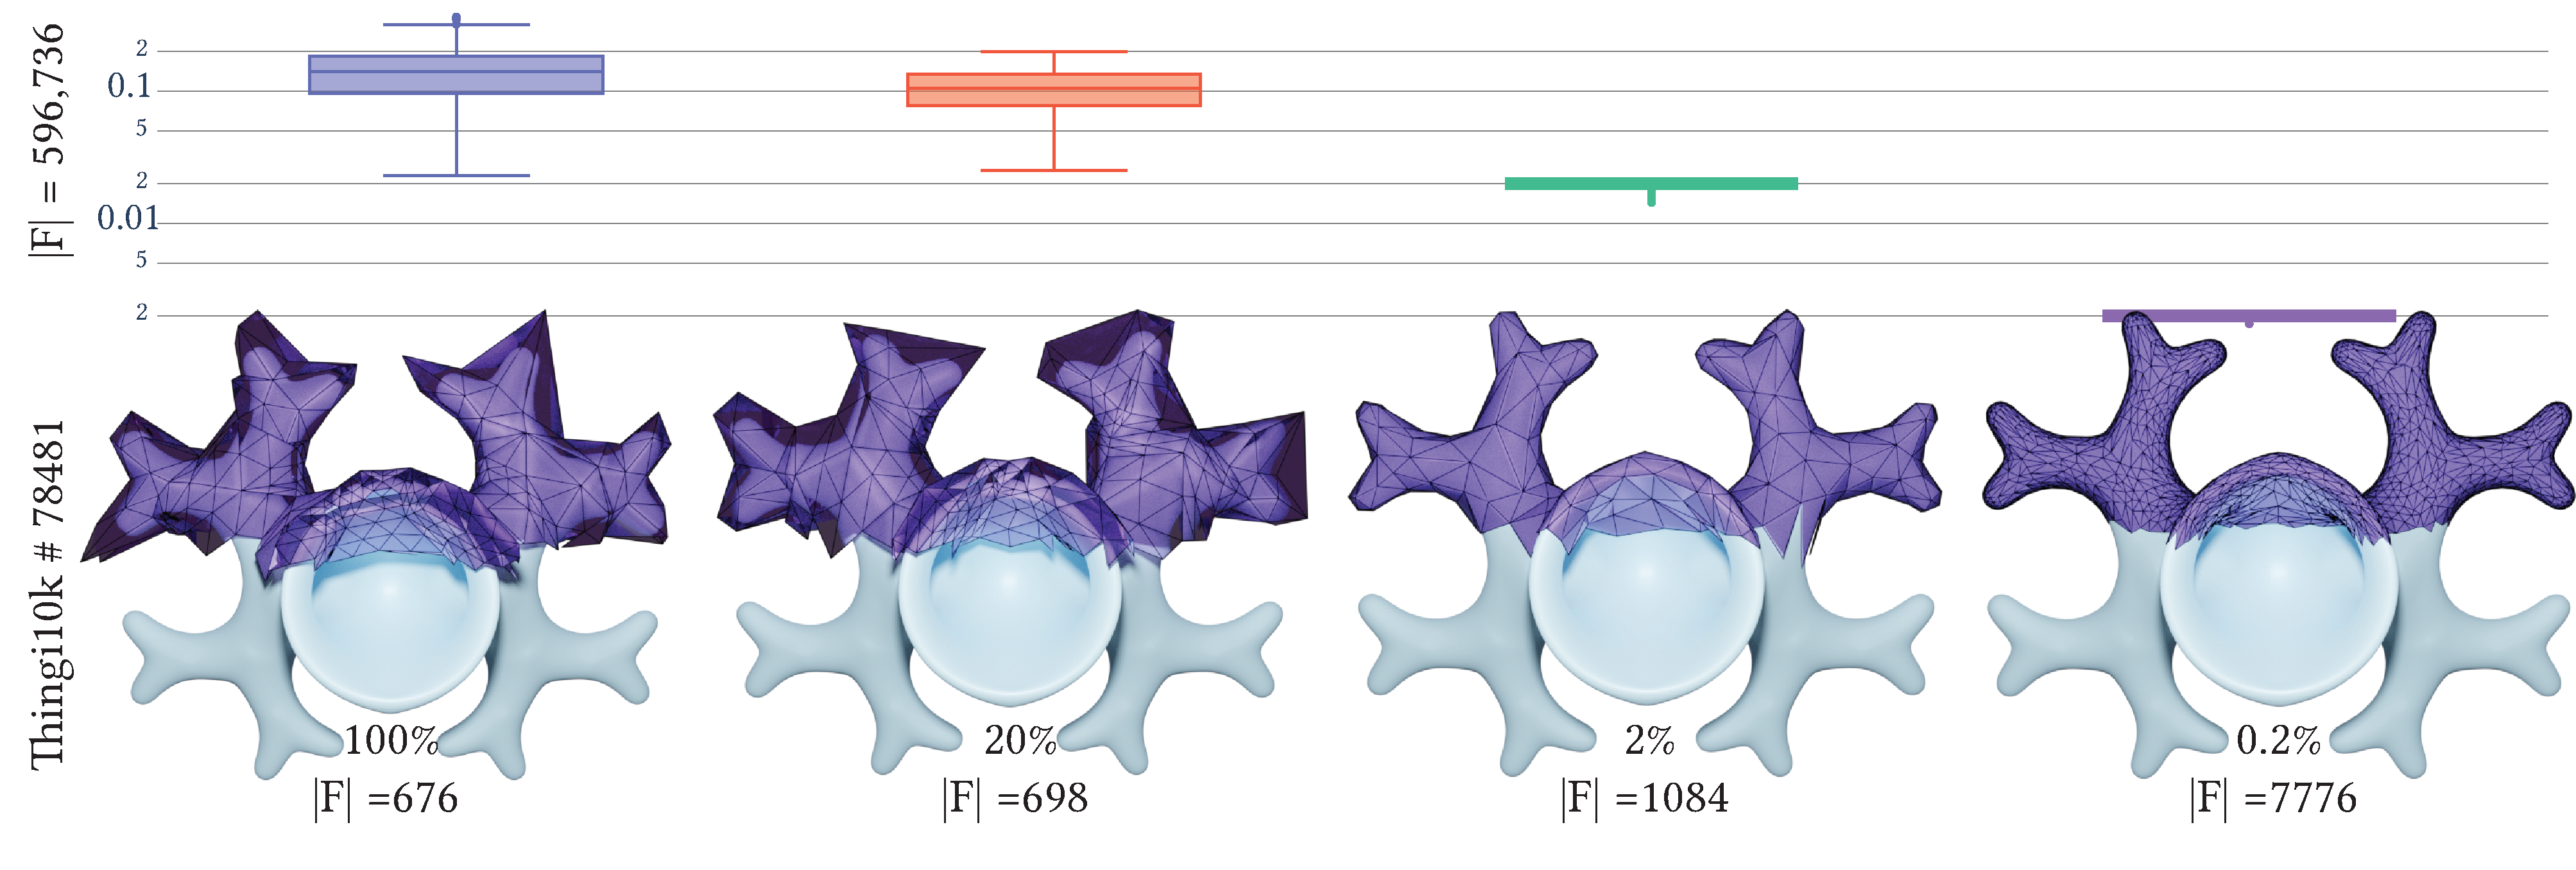
\includegraphics[width=\linewidth,draft=false]{prism-tex/figs/varying_thickness}
    %input F= 596736, Thingi10k 78481
    \caption{The effect of different target thickness on the number of prisms |F| of the final shell, 
    and distribution of final thickness (\revision{shown as the box plots on the} top).} 
    
    \label{prism:fig:vary_thick}
\end{figure}

For each dataset, we selected the subset of meshes satisfying our input assumptions:  intersection-free, orientable, manifold triangle meshes without zero area triangles (tested using a numerical tolerance $10^{-16}$).  We test self-intersections by two criteria: a ball of radius $10^{-10}$ around each vertex does not contain non-adjacent triangles; and all the dihedral angles are larger than 0.1 degrees.

We tested our algorithm on two datasets: (1) Thingi10k dataset \cite{zhou2016thingi10k} containing, after the filtering due to our input assumptions, 5018 models; and (2) the first chunk of for the ABC dataset~\cite{koch2019abc} with 5545 models.
The only user-controlled parameter of our algorithm is the target thickness of our shell; in all our experiments (unless stated otherwise), we use 10\% of the longest edge of the bounding box. 
In Figure~\ref{prism:fig:vary_thick}, we show how the target thickness influences the usage of the shell: a thicker shell provides a larger class of sections, thus accommodates more processing algorithms, while a thinner one offers a natural bound on the geometric fidelity of the sections.

% We use a large thickness in our experiments to show that our algorithm can create it, even if we expect that a thinner shell will be more practical in most applications.

\begin{figure}
    \centering
    Thingi10k\\
    \includegraphics[width=0.9\linewidth]{prism-tex/figs/10k_gallery}\\%[0.5em]
    %
    ABC\\
    \includegraphics[width=\linewidth]{prism-tex/figs/abc_gallery}
    %
    \caption{Gallery of shells built around models from Thingi10k \protect\cite{zhou2016thingi10k} and ABC~\protect\cite{koch2019abc}.}
    \label{prism:fig:gallery}
    
\end{figure}


Our algorithm successfully creates shells for all 5018 models for Thingi10k and 5545 for ABC. 
We show a few representative examples of challenging models for both datasets in Figure \ref{prism:fig:gallery}, including models with complicated geometric and topological details. In all cases, our algorithm produces coarse and thick cages, with a bijective projection field defined.

We report as a scatter plot the number of output faces, the timing, and the memory used by our algorithm (Figure \ref{prism:fig:large-dataset}).
In total, the number of prisms generated by our algorithm is 7\% and 2\% of the number of input triangles for the Thingi10k and ABC dataset respectively 
and runs with no more than 4.7 \revision{GB} of RAM. 
The generation and optimization of the shell takes 5min and 59s in average and up to 8.6 hours for the largest model. \revision{50\% of the meshes finish in 3 minutes and 75\% in 6 minutes and 15 seconds.}

% \begin{figure}
%     \centering
%     Thingi10k
%     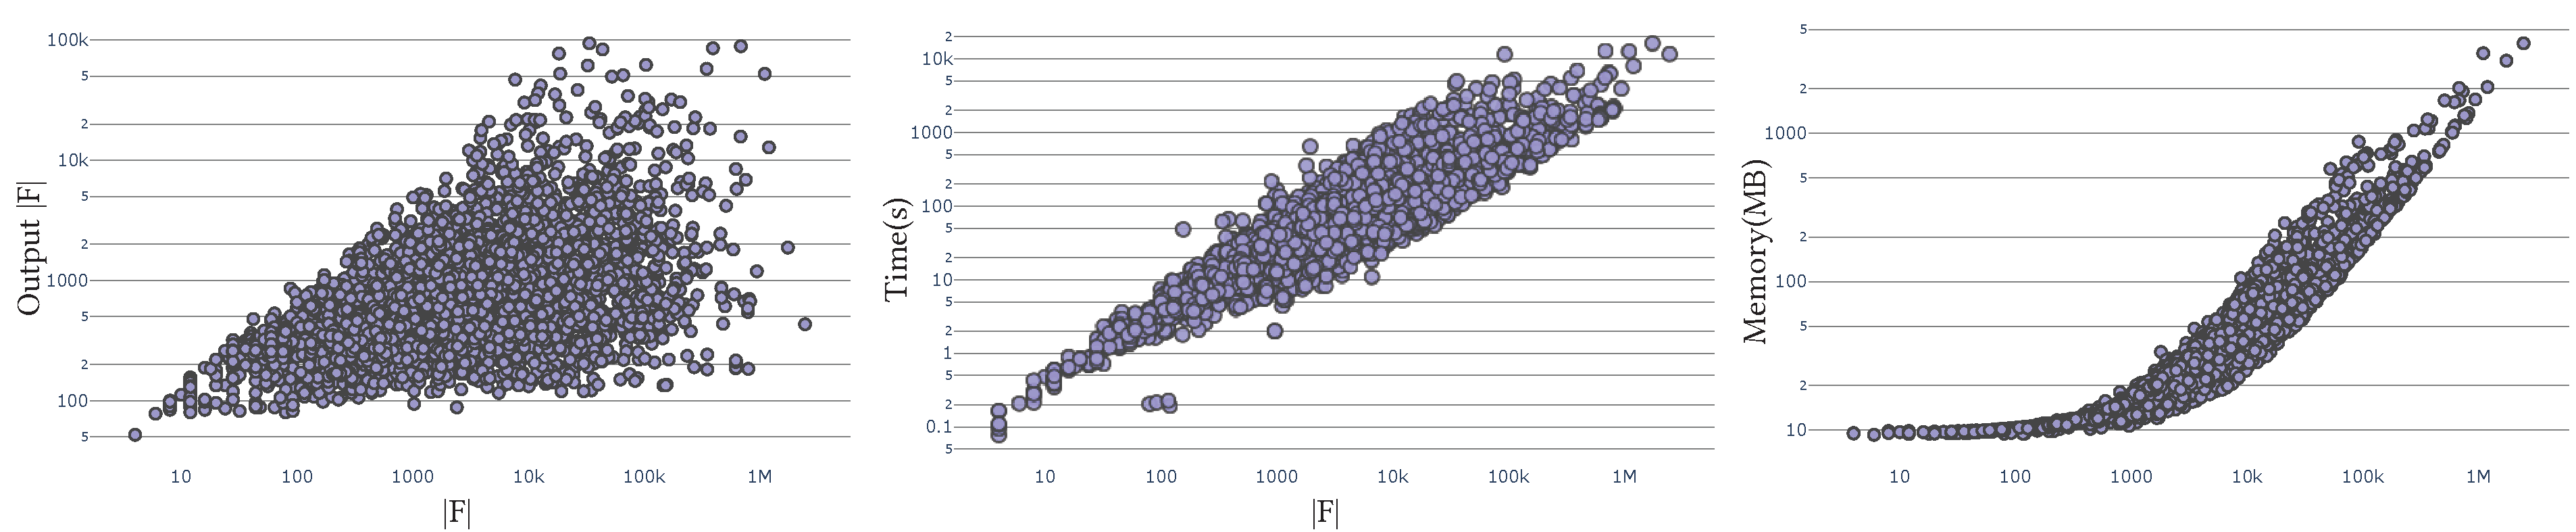
\includegraphics[width=\linewidth]{prism-tex/figs/stats10k}
%     ABC
%     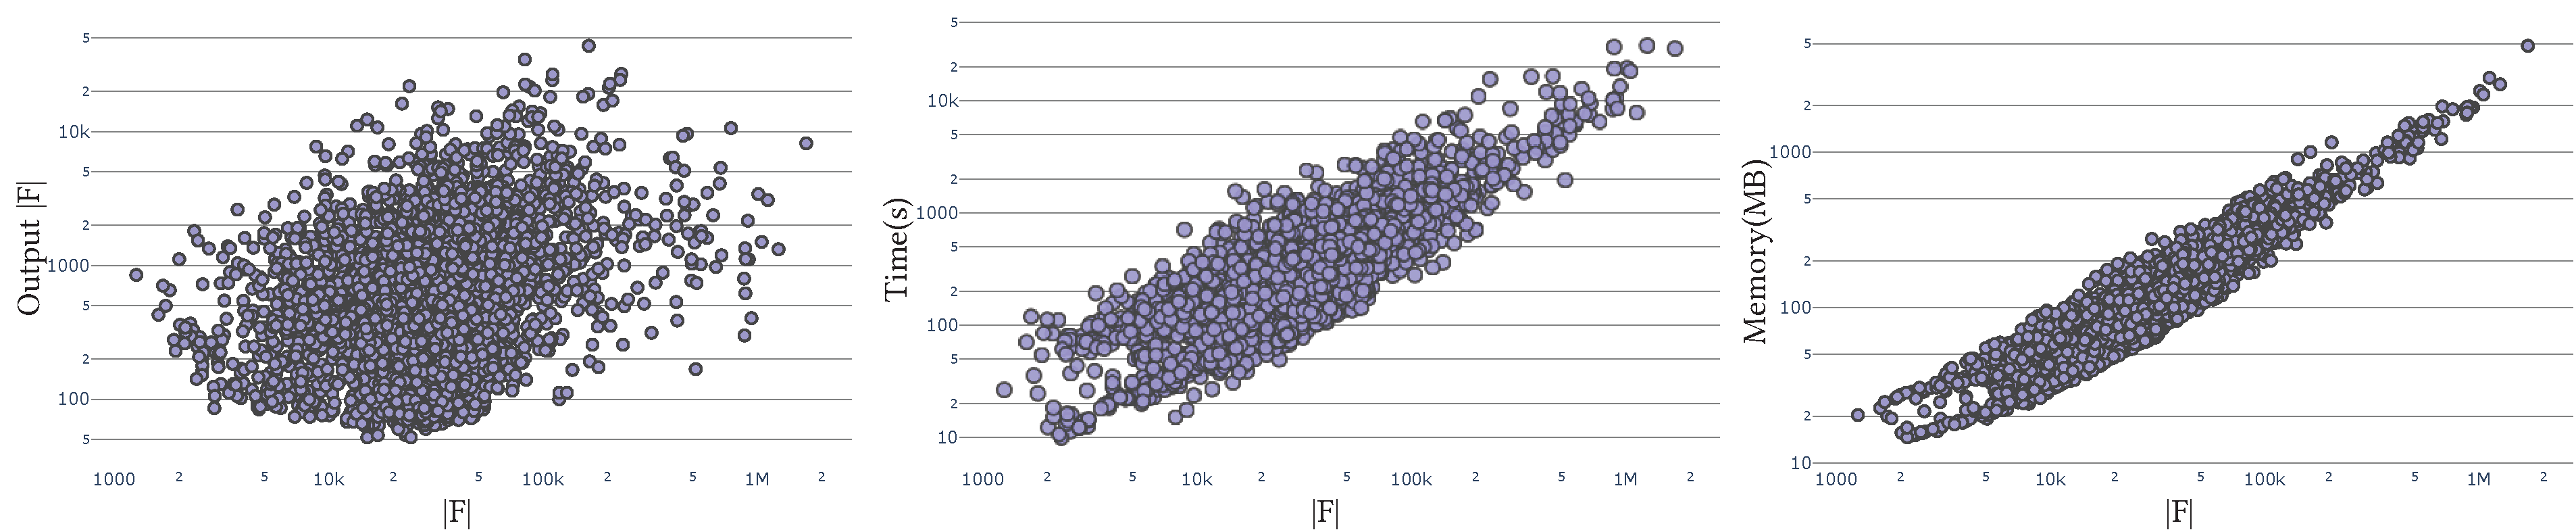
\includegraphics[width=\linewidth]{prism-tex/figs/stats_abc}
%     \caption{Statistics of 5018 shells in Thingi10k dataset \cite{zhou2016thingi10k} (top) and 5545 in ABC Dataset \cite{koch2019abc} (bottom).}
%     \label{prism:fig:large-dataset}
%     
% \end{figure}
\begin{figure}
    \centering
    \begin{tabular}{cc}
        Thingi10k & ABC \\ 
        \includegraphics[width=0.4\linewidth,page=2]{prism-tex/figs/stats_combined}
        &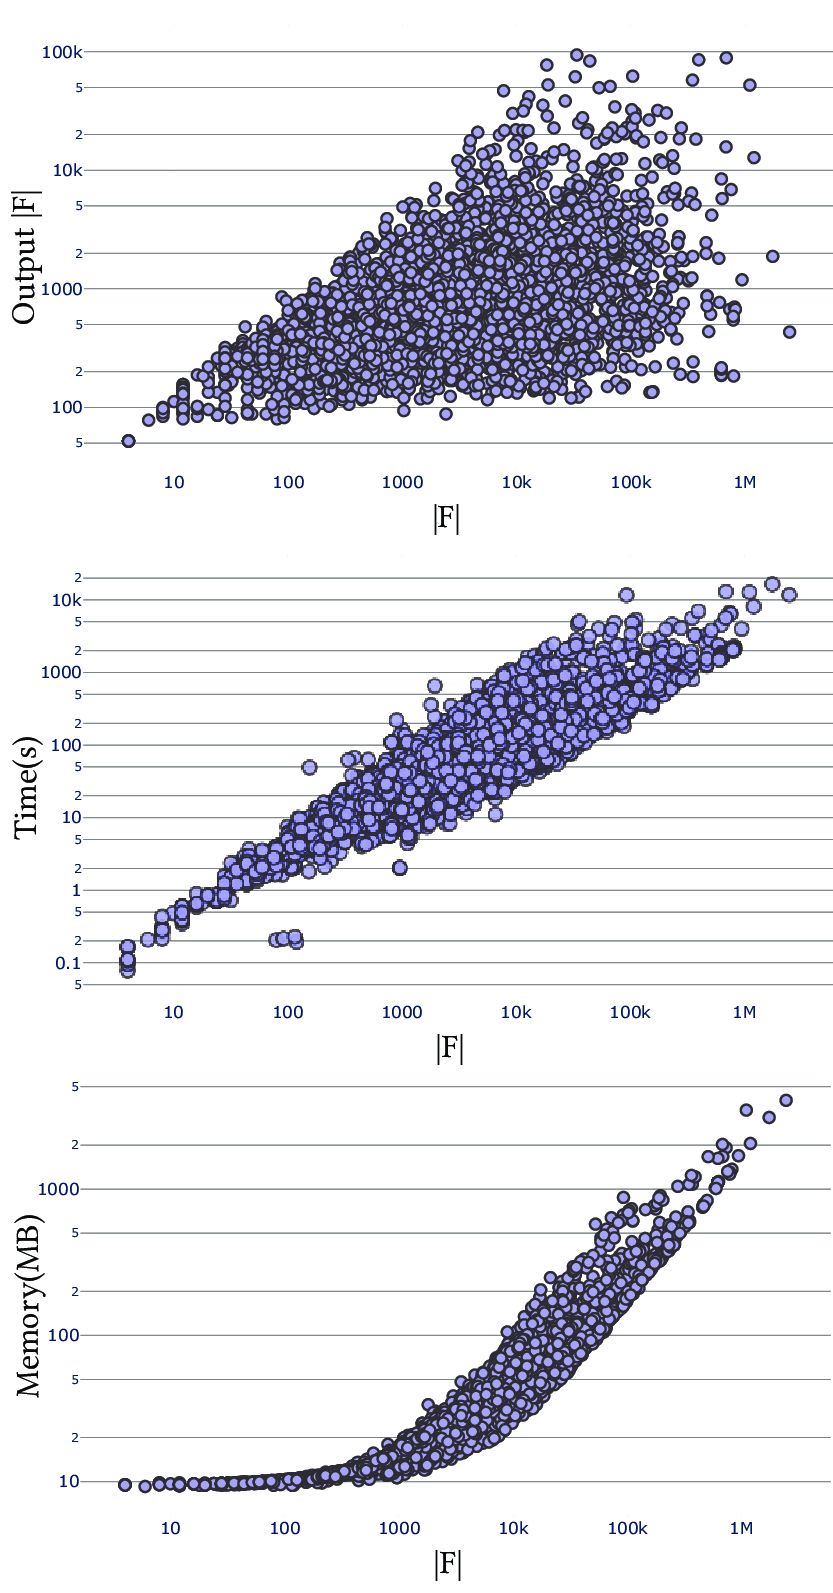
\includegraphics[width=0.4\linewidth,page=1]{prism-tex/figs/stats_combined}
    \end{tabular}
    \caption{Statistics of 5018 shells in Thingi10k dataset \cite{zhou2016thingi10k} (left) and 5545 in ABC Dataset \cite{koch2019abc} (right).}
    \label{prism:fig:large-dataset}
    
\end{figure}


\begin{figure}
    \centering
    \includegraphics[width=1\linewidth]{prism-tex/figs/thai_comparision}
    \caption{The \emph{UV based method} cannot simplify the prescribed seams, and introduces self-intersections. 
    The projection induced by the \emph{Naive Cage} method is not continuous and not bijective; it leads to visible spikes in the reconstructed geometry.}
    \label{prism:fig:qslim_naive}
    
\end{figure}

\paragraph{Comparison to Simple Baselines}
In Figure~\ref{prism:fig:qslim_naive} we compare to two baseline methods based on \cite{garland1998simplifying}. For each method, we generate a coarse mesh, uniformly subdivide it for visualization purposes, 
%this is the old text % start with a uniformly subdivided coarse mesh, 
and query the corresponding spatial position on the original input to form the subdivided mesh.
% a mesh with subdivision connectivity. 
The \emph{UV based} method is a conventional way of establishing correspondence in the context of texture mapping. However, the robust generation of a UV atlas satisfying a variety of user constraints is still an open problem. We use the state-of-the-art methods \cite{li2018optcuts,jiang2017simplicial} to generate a low-distortion bijective parametrization, and use seam-aware decimation technique~\cite{liu2017seamless} to generate the coarse mesh.
Due to the complex geometry and the length of the seam (Figure~\ref{prism:fig:qslim_naive} second figure), the simplification is not able to proceed beyond the prescribed seam while maintaining the bijectivity, making the pipeline inadequate especially for building computational domains. 
%The reconstructed geometry also exhibits excessive distortion.

\revision{We also set up a baseline of the \emph{Naive Cage} method by creating} a simplified coarse mesh with \cite{garland1998simplifying} and use Phong projection to establish the correspondence \cite{kobbelt1998interactive,panozzo2013weighted}. \revision{Such attribute transfer} is not guaranteed to be bijective; some face may not be projected (Figure~\ref{prism:fig:qslim_naive} third image). With our method, we can generate a coarse mesh while having a low-distortion bijective projection (Figure~\ref{prism:fig:qslim_naive} fourth image).

\paragraph{Numerical accuracy} 
To evaluate the numerical error introduced by  our projection operator \revision{when implemented with floating-point arithmetic}, we \emph{transfer} the vertices of the input mesh to the middle surface and \emph{inverse transfer} them from the middle surface back to the input mesh.  We measure the Euclidean distance with respect to the source vertices (Figure~\ref{prism:fig:shark_accuracy}). 
We compare the same experiment with the Phong projection \cite{kobbelt1998interactive}. This alternative approach exhibits distance errors up to $10^{-5}$ even after ruling out the outliers for which the method fails due to its lack of bijectivity.  The maximal error of our projection is on the order of $10^{-8}$; this error could be completely eliminated (for applications requiring an exact bijection) by implementing the projection operator and its inverse using rational arithmetic.
\begin{figure}
    \centering
    \includegraphics[width=\linewidth]{prism-tex/figs/shark_accuracy}
    \caption{Our projection is three orders of magnitude more accurate than the baseline method, and bijectively reconstructs the input vertex coordinates.}
    \label{prism:fig:shark_accuracy}
    
\end{figure}
%%%%%%%%%%%%%%%%%%%%%%%%%%%%%%%%%%%%%%%%%%%%%%%%%%%%%
%%%%%%%%%%%%%%%%%%%%%%%%%%%%%%%%%%%%%%%%%%%%%%%%%%%%%
%%%%%%%%%%%%%%%%%%%%%%%%%%%%%%%%%%%%%%%%%%%%%%%%%%%%%
%%%%%%%%%%%%%%%%%%%%%%%%%%%%%%%%%%%%%%%%%%%%%%%%%%%%%
\section{Applications}
\label{prism:sec:applications}
Using our shell $\S$, we implement the following predicates and functions:
\begin{itemize}
    \item $\isinside(p)$: returns true if the point $p \in \mathbb{R}^3$ is inside $\S$. %\TS{and there is only one prism containing $p$}
    \item $\issection(\T)$: returns true if the triangle mesh $\T$ is a section of $\S$.
    % \item $\P_\T(t_{id},\alpha,\beta)$: returns the prism id and the barycentric coordinates  of the projection of the vertex of $\T$ in the triangle tid, at barycentric coordinates $\alpha$,$\beta$
    \item $\P(p)$: returns the prism id (pid), the barycentric coordinates ($\alpha,\beta$) \revision{in the corresponding triangle of the middle surface}, \revision{and the relative offset distance from the middle surface 
    ($h$, which is -1 for the bottom surface, and 1 for the top surface) of the projection of the point $p$.}
    \item $\P^{-1}(\text{pid},\alpha,\beta,h)$ is the inverse of $\P(p)$.
    \item \revision{$\P_\T(\text{tid}, \alpha,\beta) = \P(q)$, where $q$ is the point in the triangle tid of the mesh $\T$ , with barycentric coordinates $\alpha,\beta$.}
    \item \revision{$\P_\T^{-1}(\text{pid},\alpha,\beta)$ is the inverse of $\P_\T$.}
\end{itemize}

As explained in Section~\ref{prism:sec:method}, our shell may self-intersect and 
%to avoid keeping track of the correspondences, 
we opted to simply exclude the overlapping regions. In practice this affects only the function $\isinside(p)$ which needs to check if $p$ is contained in two or more non-adjacent prisms. 

These functions are sufficient to implement all applications below, demonstrating the flexibility of our construction and how easy it is to integrate in existing geometry processing workflows. %We used a floating-point version of these functions for performance reasons, but we will also provide a slower, yet exact, version for applications that require strict bijectivity.

%%%%%%%%%%%%%%%%%%%%%%%%%%%%%%%%


\begin{figure}
    \centering
    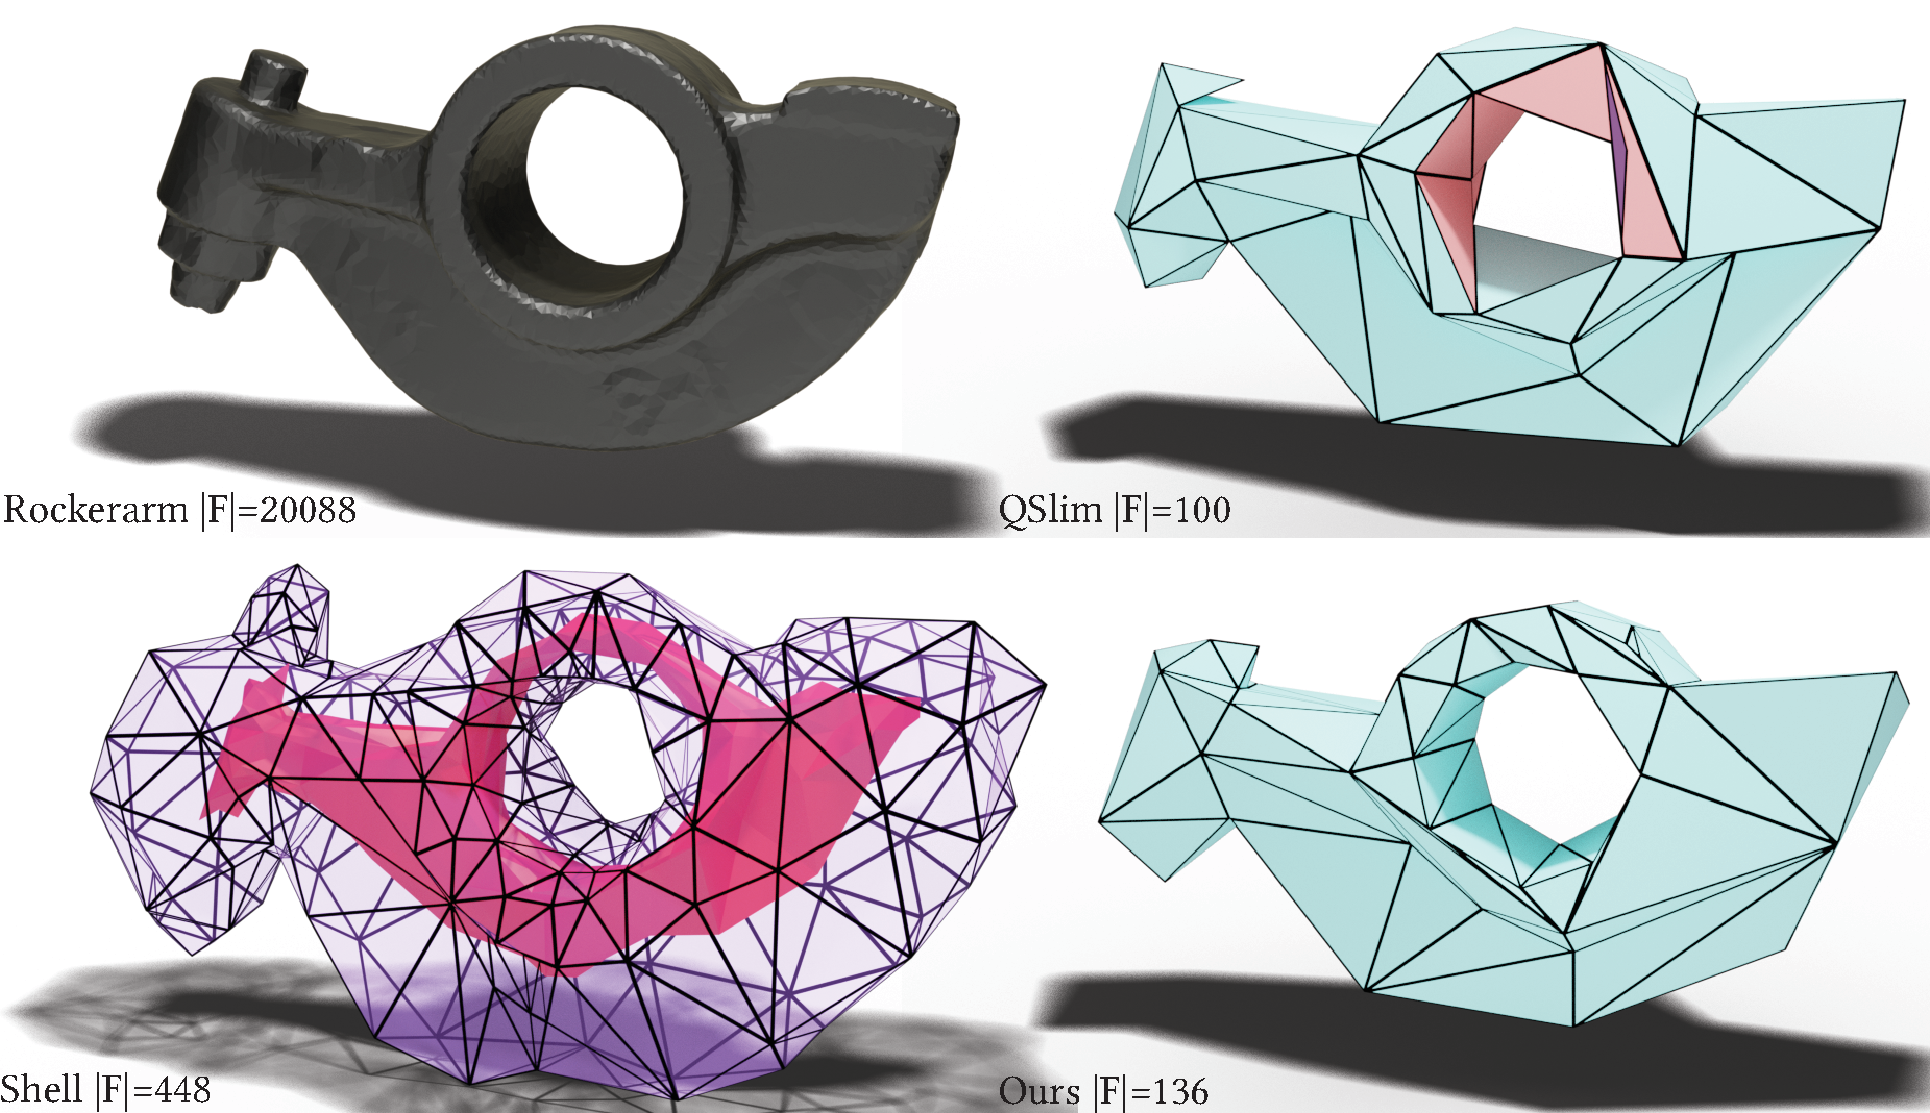
\includegraphics[width=1\linewidth]{prism-tex/figs/rockerarm_qslim}
    \caption{We attempt to simplify \protect\emph{rockerarm} (top left) from 20088 triangles to 100. QSlim~\cite{garland1998simplifying} succeeds in reaching the target triangle count (top right) but generates an output with a self-intersection (red) and flipped triangles (purple).
    With our shell constraints (bottom left), the simplification stagnates at 136 triangles, but the output is free from undesirable geometric configurations. \revision{Note that both examples use the same quadratic error metric based sceduling~\cite{garland1998simplifying}.}
    }
    % 868 Distortion Reject, 284 Intersection Reject.
    \label{prism:fig:qslim100}
    
\end{figure}

\paragraph{Remeshing}
We integrated our shell in the meshing algorithm proposed in \cite{dunyach2013adaptive} by adding envelope checks ensuring that the surface is a section after every operation. After simplification, we can use the projection operator to transfer properties between the original and remeshed surface (e.g., figures \ref{prism:fig:proxy-heat}, \ref{prism:fig:proxy-tetgen}).
%During the algorithm, we can also transfer sharp features to the current surface \DP{How is it done?} to preserve them in the remeshed surface (Figure \ref{prism:fig:sharp}).
Since the  remeshed surface is a section, a very practical side effect of our construction is that the remeshed surface is \emph{guaranteed to be free of self-intersections}, 
% \ZJ{the next sentence is commented out}
As shown in Figure~\ref{prism:fig:qslim100}, the constraints enforced through our shell prevents undesirable geometric configurations (intersections, pockets, or triangle flips).

%boundaries are preserved by our algorithm during shell construction, but cannot be simplified without breaking the bijectivity of the map. For applications such as remeshing, it is easy to allow the boundary to be simplified by enabling also the points on the boundary to move (Figure \ref{}), and the locally injective map from the remeshed surface to the input can still be used to resample attributes.


%%%%%%%%%%%%%%%%%%%%%%%%%%%%%%%%
\begin{figure}
    \centering
    \includegraphics[width=\linewidth]{prism-tex/figs/heat-in-nut}
    \caption{The heat method (right top) produces inaccurate results due to a poor triangulation (left top). We remesh the input with our method (left bottom), compute the \revision{solution of the heat method~\cite{crane2013geodesics}} on the high-quality mesh (middle bottom) and transfer the solution back to the input mesh using the bijective projection (bottom right). This process produces a result closer to the exact discrete geodesic distance \cite{mitchell1987discrete} (top middle, \revision{error shown in the histograms}).}
    \label{prism:fig:proxy-heat}
    
\end{figure}


\begin{figure}
    \centering
    \includegraphics[width=\linewidth]{prism-tex/figs/tet-knot}
    \caption{\emph{Knot} simplified with our method and tetrahedralized with TetGen. 
    The original model is converted to 1,503,428 tetrahedra (left) while the simplified surface is converted to only
    176,190 tetrahedra (right).}
    \label{prism:fig:proxy-tetgen}
    
\end{figure}


\paragraph{Proxy}
A particularly useful application of our shell is the construction of proxy domains for the solutions of PDEs on low-quality meshes. 
Additionally, by specifying the target thickness parameter (Figure~\ref{prism:fig:vary_thick}),
we are able to bound the geometry approximation error to the input as well.
Using our method,
we can (1) convert a low-quality mesh to a proxy mesh with higher quality and desired density, (2) map the boundary conditions from the input to the proxy using the bijective projection map, (3) solve the PDE on the proxy (which is a standard mesh), and (4) transfer back the solution on the input surface (Figure \ref{prism:fig:proxy-heat}). 
% \ZJ{NiT discussion is commented out below.}
\revision{Our} algorithm can be directly used to solve volumetric PDEs.
by calling an existing tetrahedral meshing algorithm between steps 2 and 3 (figures \ref{prism:fig:teaser},~\ref{prism:fig:proxy-tetgen}). 
In this case, we control the geometric error by setting the target thickness (we use 2\% of the longest edge of the bounding box).

% \begin{figure}
%     \centering
%     \includegraphics[width=1\linewidth]{prism-tex/figs/uvsphere-nit}
%     \caption{Intrinsic refinement~\cite{sharp2019navigating} cannot simplify the input mesh, while our approach can freely change the input connectivity and resolution. We can create a high-quality, isotropic triangulation of the sphere by uniformly upsampling the middle surface and projecting it to the input with our projection. Note that this mesh is a section, and we can thus transfer any attribute from the input bijectively.}
%     \label{prism:fig:uvsphere_nit}
% \end{figure}

%%%%%%%%%%%%%%%%%%%%%%%%%%%%%%%%

\begin{figure}
    \centering
    \includegraphics[width=0.9\linewidth]{prism-tex/figs/birdengine}
    \caption{The union of two meshes is coarsened through our algorithm, while preserving the exact correspondence, as shown through color transfer.}
    \label{prism:fig:birdengine}
    
\end{figure}

\paragraph{Boolean Operations}
The mesh arrangements algorithm enables the robust and exact (up to a final floating-point rounding) computation of Boolean operations on PWN meshes \cite{zhou2016mesh}. 
However, the produced meshes tend to have low triangle quality that might hinder the performance of \revision{downstream} algorithms. %using them to evaluate large CSG trees. 
By interleaving a remeshing step performed with our algorithm after every operation, we ensure  high final quality and more stable runtime. The composition of the bijections enables us to transfer properties between different nodes of the CSG tree (Figure~\ref{prism:fig:birdengine}).%\ZJ{I am not sure we want to talk about CSG tree, since we did not really have it.}


%%%%%%%%%%%%%%%%%%%%%%%%%%%%%%%%
\begin{figure}
    \centering
    \includegraphics[width=0.95\linewidth]{prism-tex/figs/bunny-displacement}
    \caption{Top: an input mesh decimated to create a coarse base mesh, and the details are encoded in a displacement map (along the normal) with correspondences computed with Phong projection \cite{kobbelt1998interactive}. Bottom: the decimation is done within our shell while using the same projection as above. With our construction, this projection becomes bijective (Appendix \ref{app:bilinear}), avoiding the artifacts visible on the ears of  the bunny in the top row.}
    \label{prism:fig:displacement-mapping}
    
\end{figure}
\paragraph{Displacement Mapping}
The middle surface of the shell is a coarse triangular mesh that can be directly used to compress the geometry of the input mesh, storing only the coarse mesh connectivity and adding the details using normal and displacement maps (Figure \ref{prism:fig:displacement-mapping}). A common way to build such displacement is to project \revision{\cite{kobbelt1998interactive,collins2002mesh}} the dense mesh on the coarser version. As shown in Appendix \ref{app:bilinear}, our method guarantees that this natural projection is also bijective as long as the coarse mesh is a section. This 
\revision{alleviates the loss of information}
% ensures that no information is lost 
even on challenging geometry configurations, and our shell can thus be used to automate the creation of projection cages and displacement maps.
%%%%%%%%%%%%%%%%%%%%%%%%%%%%%%%%

% \paragraph{Boundary Layers}
% Boundary layer meshes are commonly used in computational fluid dynamics. Our algorithm can be used to generate them by sampling the inverse projection operator at different heights to construct a set of thinner prismatic layers (Figure \ref{}). The volume outside of the shell can then be meshed using TetGen \cite{}.


%%%%%%%%%%%%%%%%%%%%%%%%%%%%%%%%
\begin{figure}
    \centering
    \includegraphics[width=\linewidth]{prism-tex/figs/chain-lizard}
    \caption{Two volumetric chainmail textures (right) are applied to a shell (bottom left) constructed from the \emph{Animal} mesh (top left).
    The original UV coordinates are transferred using our projection operator.}
    \label{prism:fig:volumetric-textures}
    
\end{figure}
\paragraph{Geometric Textures.}
The inverse projection operator provides a 2.5D parametrization around a given mesh and can be used to apply a volumetric texture (Figure \ref{prism:fig:volumetric-textures}).
Note that we build the volumetric texture on the simplified shell, while still being able to bijectively transfer the texture coordinates.
%We also believe our discussion on the valid shells (Section~\ref{prism:sec:singularities}) will be the building block for a robust shell map algorithm.}



%%%%%%%%%%%%%%%%%%%%%%%%%%%%%%%%%%%%%%
%%%%%%%%%%%%%%%%%%%%%%%%%%%%%%%%%%%%%%
%%%%%%%%%%%%%%%%%%%%%%%%%%%%%%%%%%%%%%



\section{Variants}\label{prism:sec:variants}


\paragraph{Input with Self-Intersections}
Up to this point, we assumed that our input meshes are without self-intersections. This requirement is necessary to guarantee a bijection between any section (e.g., the input mesh) and the middle surface. Such bijection is essential for a key target application, the transfer of boundary conditions for solving PDEs on meshes or mesh-bounded domains. 

However, our method can be easily extended to meshes containing self-intersections, broadening the class of meshes it can be applied to, at the cost of making the resulting shell usable in fewer application scenarios: for example, if it is used for remeshing, it will likely generate a new surface that still contains self-intersections.

If $\T$ contains self-intersections, our algorithm can be trivially extended to generate a shell which will be \emph{locally injective}, and the bijectivity of the mapping between sections still holds but with respect to the immersion. The only change required is to modify the invariance checks (Section \ref{prism:sec:optimization}): we have to replace the global intersection check with checking whether local triangles overlap with the current prisms. Figure~\ref{prism:fig:intersect-leg} shows an example of a mesh $\T$ with self-intersections, the generated shell, and the isolines of geodesic transferred on the coarser middle surface.
\begin{figure}
    \centering
    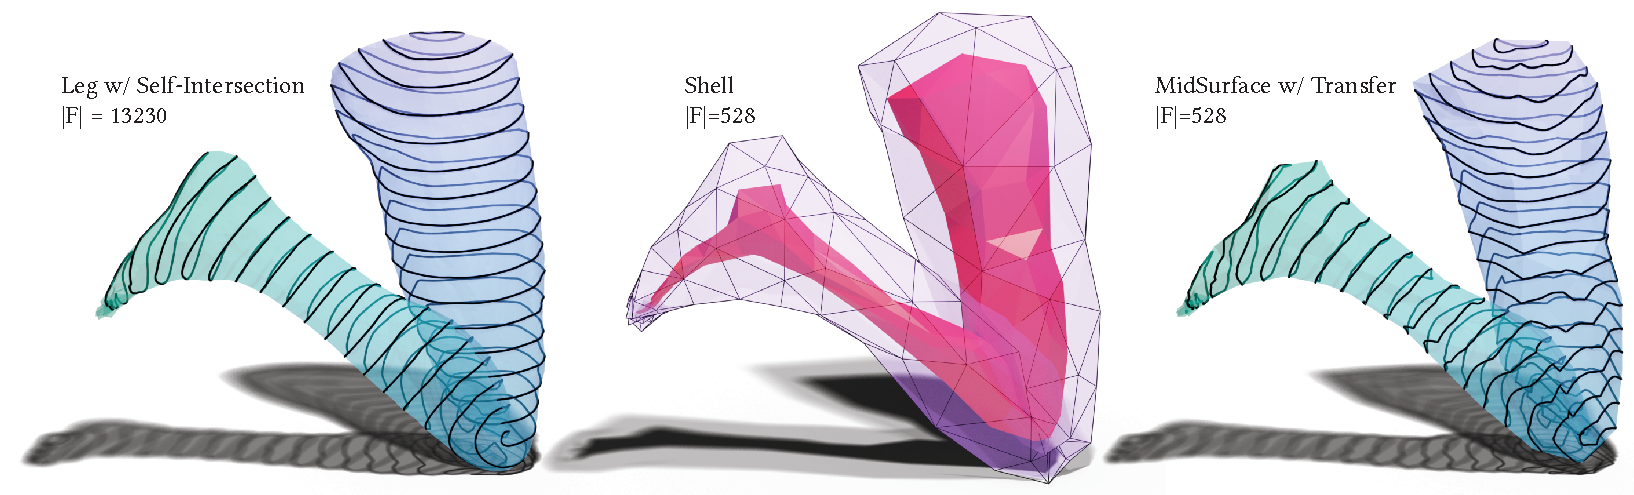
\includegraphics[width=\linewidth]{prism-tex/figs/leg-intersect}
    \caption{An example of a shell built around a self-intersecting mesh.}
    \label{prism:fig:intersect-leg}
    
\end{figure}


\begin{figure}
    \centering
    \includegraphics[width=\linewidth]{prism-tex/figs/armadillo_cage}
    \caption{The \protect\emph{Armadillo} model with four nested cages. We create a shell from the original mesh, and then rerun our algorithm on the outer shell to create the other three layers. Note that all layers are free of self-intersections, and we have an explicit bijective map between them.}
    
    \label{prism:fig:nested-cages}
\end{figure}

\paragraph{Resolving Shell Self-Intersections}
\label{prism:sec:postprocessing}
% During initialization and optimization, we forbid the top and bottom surfaces to intersect with $\T$. However, the optimized shell $\S$ might have self-intersections, i.e. there can be a point in ambient space contained in more than one prism.  While this is not an issue for our shell construction and optimization (which is defined inside every prism), this is not desirable for specific applications 
% where the offset surface we created for geometry processing tasks. 
For certain applications it might be preferable to have a shell whose  \revision{top and bottom surfaces do} not self-intersect:
for example, in the construction of nested cages \cite{sacht2015nested} (useful for collision proxies and animation cages), we want to iteratively build nested shells while ensuring no intersections between them (Figure \ref{prism:fig:nested-cages}). 
With a small modification, our algorithm can be used to generate nested cage automatically and robustly, with the additional advantage of being able to map any quantity  bijectively across the layers and to the input mesh. In contrast, \cite{sacht2015nested}
does not provide guarantees on the success (e.g., the reference implementation of \cite{sacht2015nested} fails on Figure~\ref{prism:fig:qslim_naive}, probably due to the presence of a singularity). 
\begin{figure}
    \centering
    \includegraphics[width=0.8\linewidth]{prism-tex/figs/camel}
    \caption{After optimization, the shell may self-intersect (left). Our postprocessing can be used to extract a non-selfintersecting shell, which is easier to use in downstream applications (right).}
    \label{prism:fig:shell_shrinking-cages}
    
\end{figure}

To resolve the self-intersections of the top (bottom) surface, we identify the regions covered by more than one prism by explicitly testing intersections between the tetrahedralized prisms, accelerated using \cite{zomorodian2000fast}. For every detected prism, we reduce the thickness by 20\%, and iterate until no more intersections are found. 
Differently from the procedure in Section \ref{prism:sec:initialization}, where reducing the thickness of the shell always maintains the validity of the shell, at this stage, the shrinking of the shell may make the shell invalid, since $\T$ may not be contained anymore in $\S$. 
Whenever this happens, we perform one step of red-green refinement \cite{bank1983some} on the regions we wish to thin, and we iterate until we succeed. This procedure is guaranteed to terminate since, on the limit of the refinement, the middle surface will be geometrically identical to $\T$, and thus Theorem \ref{thm:thickness} holds.
In the worst case, the procedure terminates when the size of triangles on the middle surface is comparable to the input; then no refinement is required to shrink below the minimum separation of the input.
Figure~\ref{prism:fig:shell_shrinking-cages} shows how the intersecting shell between the legs of the camel can be shrunk to generate an intersection-free shell. 



\begin{figure}
    \centering
    \includegraphics[width=0.9\linewidth]{prism-tex/figs/blocks}
    \caption{We generate a pinched shell for a model with a singularity (left).
    Optionally, we can complete the shell using our Boolean construction.}
    \label{prism:fig:singularity-boolean}
    
\end{figure}


\paragraph{Pinching Alternative.} For certain applications, such as boundary layer meshing, it is necessary to have a shell with non-zero thickness everywhere, including at singularities, and it is tolerable to lose bijectivity at the vicinity of a singularity. For these cases, we propose a Boolean construction to \emph{fill} the shell around singularities, and to extend the projection operator $\P$ inside these regions. That is, every point in the filled region will project to the singularity. 
% An unavoidable (with our definition of projection) side effect of this construction is that $\P$ loses local injectivity.

Without loss of generality, let us assume that $\T$ has a single singularity (Figure \ref{prism:fig:singularity-boolean}). We initially construct a pinched shell, with zero thickness at the singularity, construct a valid shell (Section~\ref{prism:sec:method}), and then perform a corefinement~\cite{corefinement} between a tetrahedron (centered at the singularity and whose size is smaller than the minimal thickness of the neighboring vertices) and the shell. The result of the corefinement operation (Figure \ref{prism:fig:singularity-boolean} middle) consists of triangles belong to the tetrahedron, or the shell surface. The remaining part of the tetrahedron is a star-shaped polyhedron with the singularity in its kernel, and sharing a part of its boundary with the shell. This polyhedron can be easily tetrahedralized by connecting its triangulated boundary faces (one of them is highlighted in red in Figure \ref{prism:fig:singularity-boolean} middle) with the singularity. For every point $p$ in these tetrahedra, the projection operator $\P$ projects $p$ to the singularity. The remaining triangles are divided into two groups: 
the triangles with only one new vertex complete the degenerate prisms (one of them is highlighted in blue in Figure \ref{prism:fig:singularity-boolean} middle), 
while the others map to the edges they are attached to.





